\section{Diagrama}
Neste segundo experimento, introduzimos ruído branco gaussiano dentro do canal e modelamos a atenuação sofrida pelo sinal durante o percurso, de forma que possamos observar a deterioração da Taxa de Erro de Bit e o espalhamento dos pontos da constelação QPSK. O esquema de modulação continua exatamente o mesmo.  

\begin{figure}
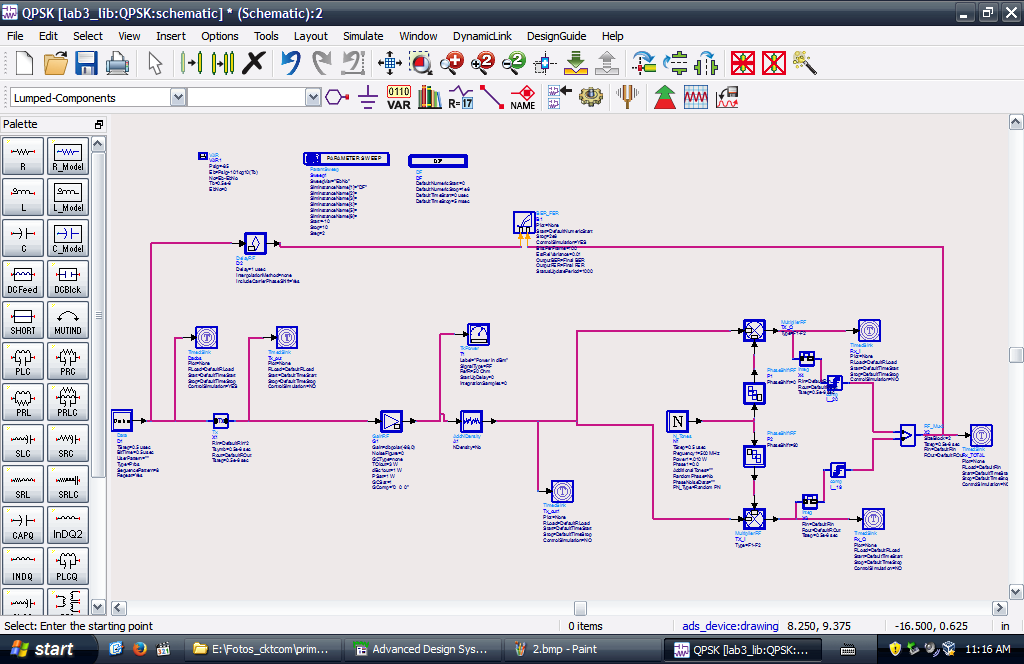
\includegraphics[width=.7\linewidth]{./segundo_exp/1.png}
\caption{Diagrama de Blocos Referente ao Segundo Experimento}
\end{figure}


\section{Resultados}
Como esperado, a medida que a relação $E_b/N_o$ que é análoga a SNR se deteriora, a Taxa de Erro de bit aumenta até se aproximar do seu valor limite de 0,5. A nuvem de pontos da constelação QPSK também fica cada vez mais espalhada na medida em que a relação se deteriora.


\begin{figure}
\centering
\begin{minipage}{.48\textwidth}
  \centering
  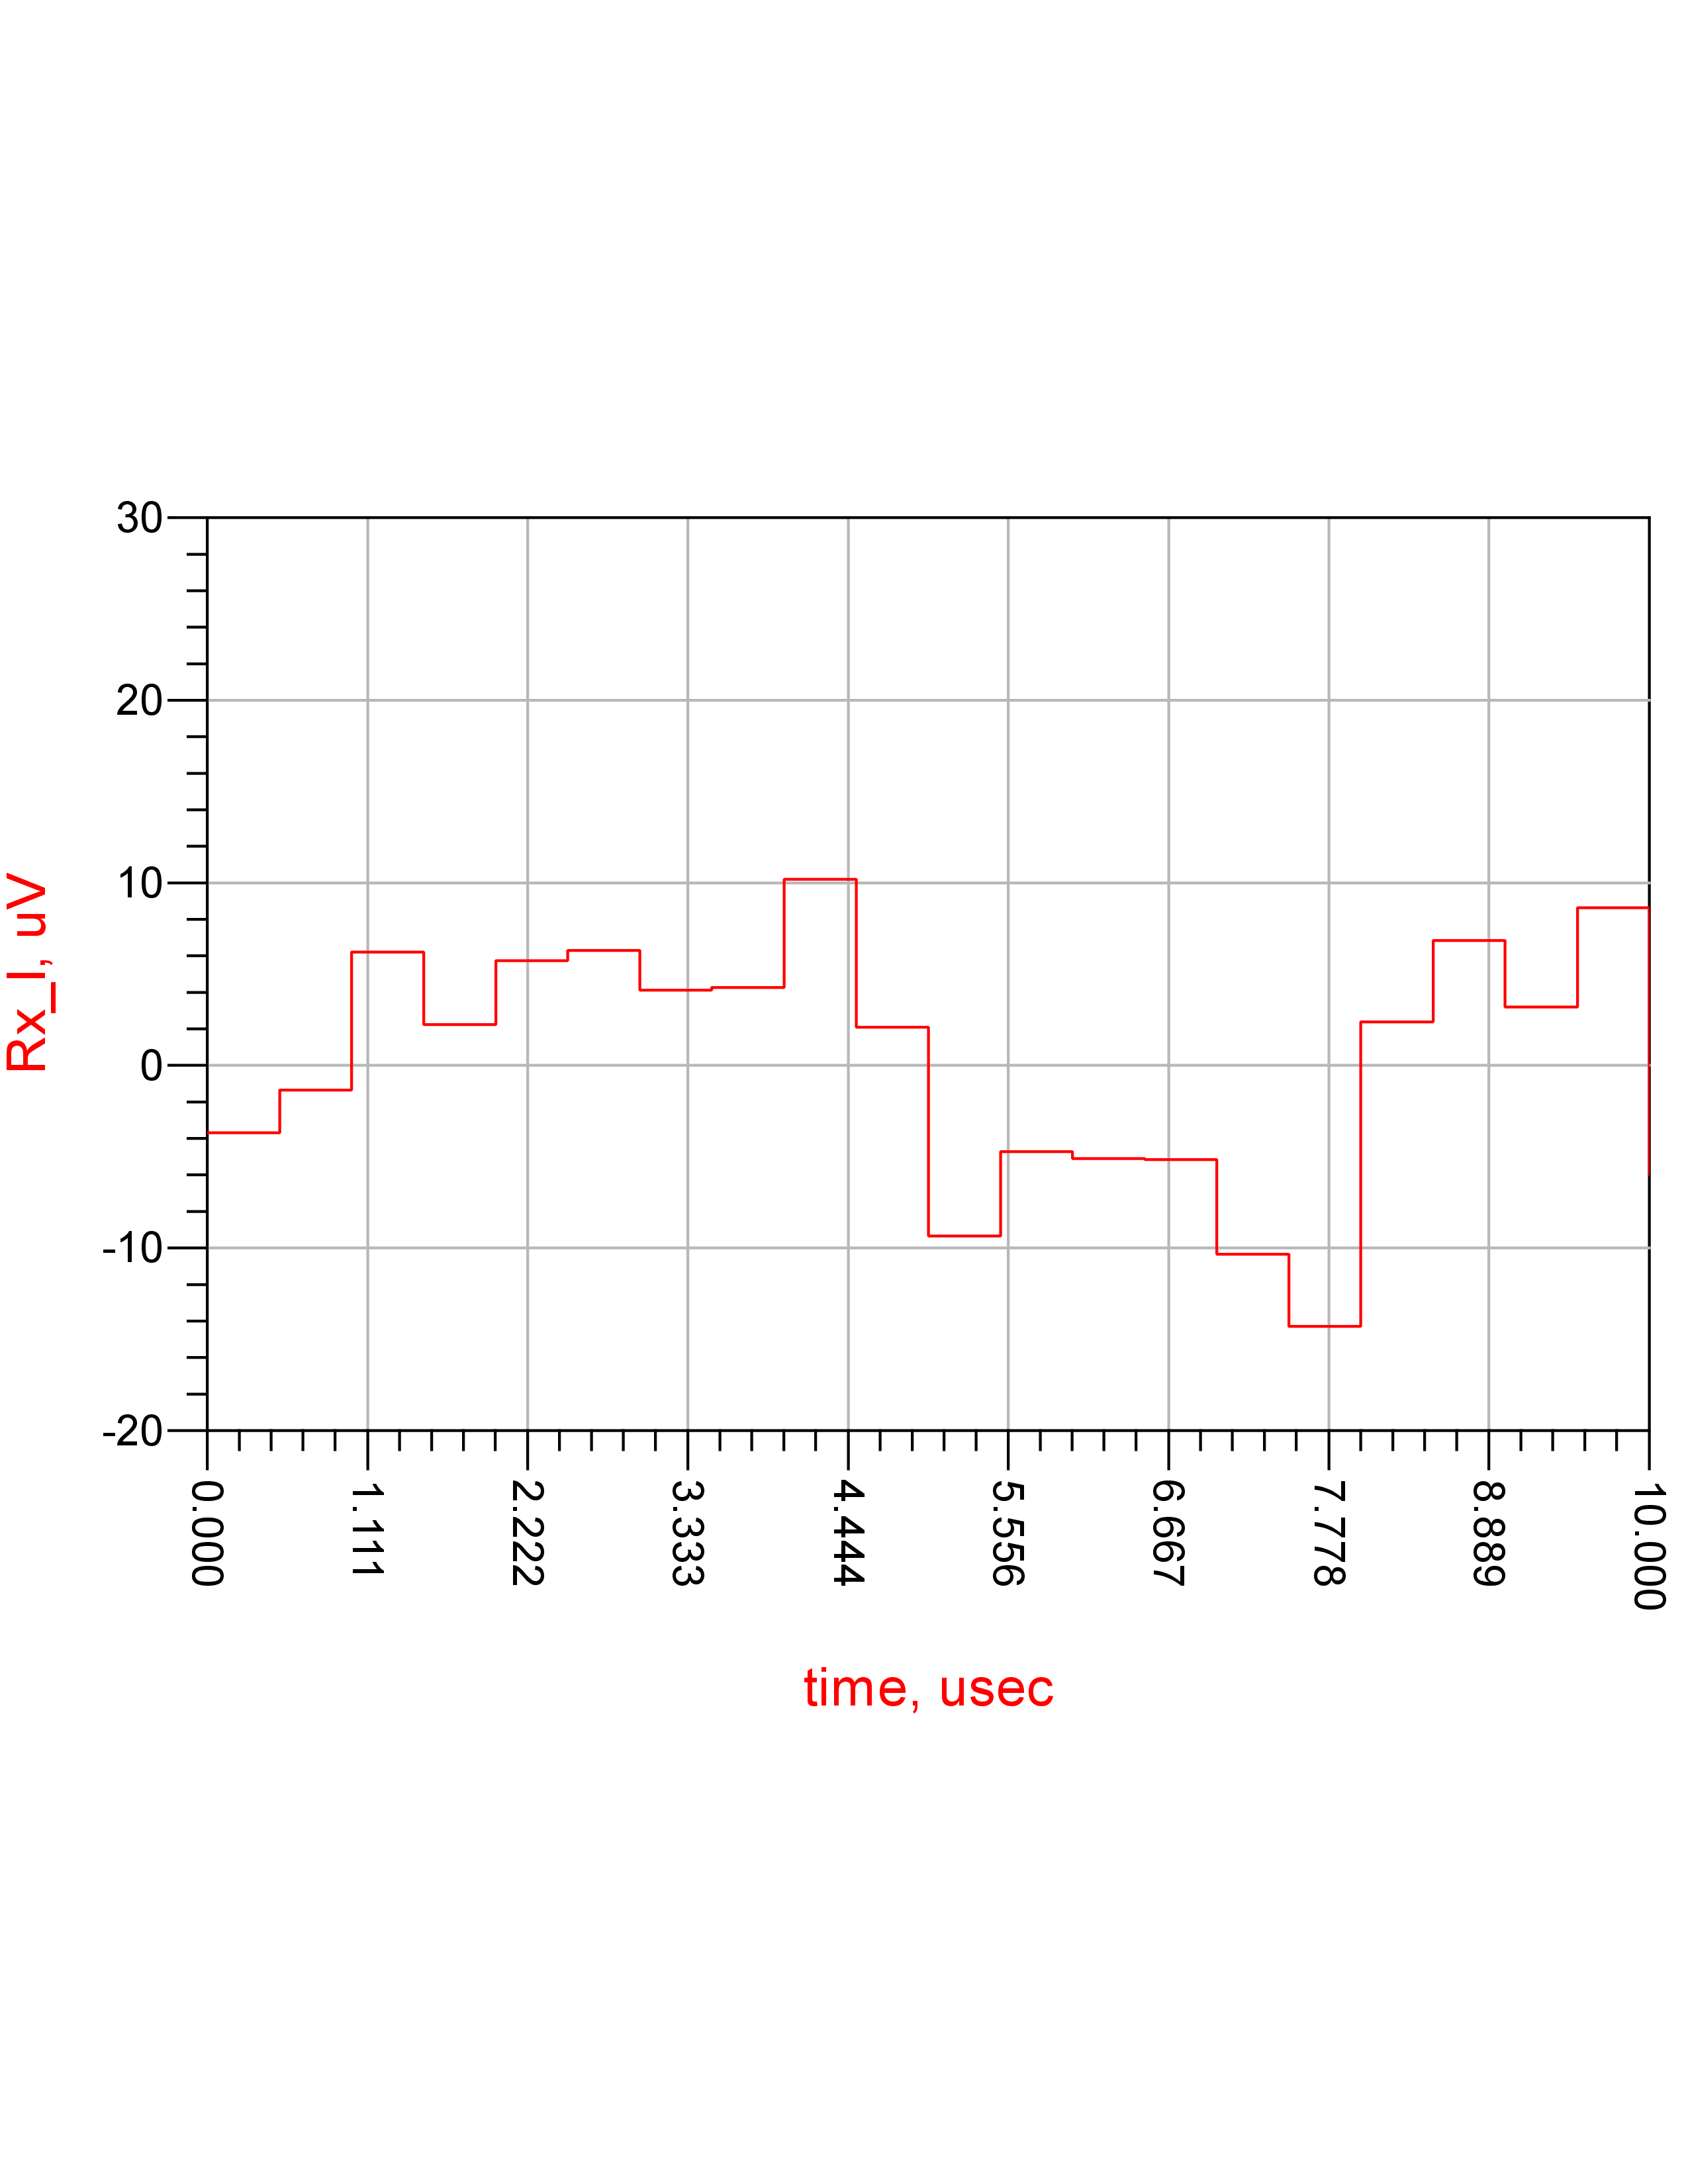
\includegraphics[width=\linewidth]{./segundo_exp/img4.png}
  \captionof{figure}{Via I, vemos os dados fortemente afetados pelo ruído e atenuação impostas}
  \label{fig:test38}
\end{minipage}%
  \hfill
\begin{minipage}{.48\textwidth}
  \centering
  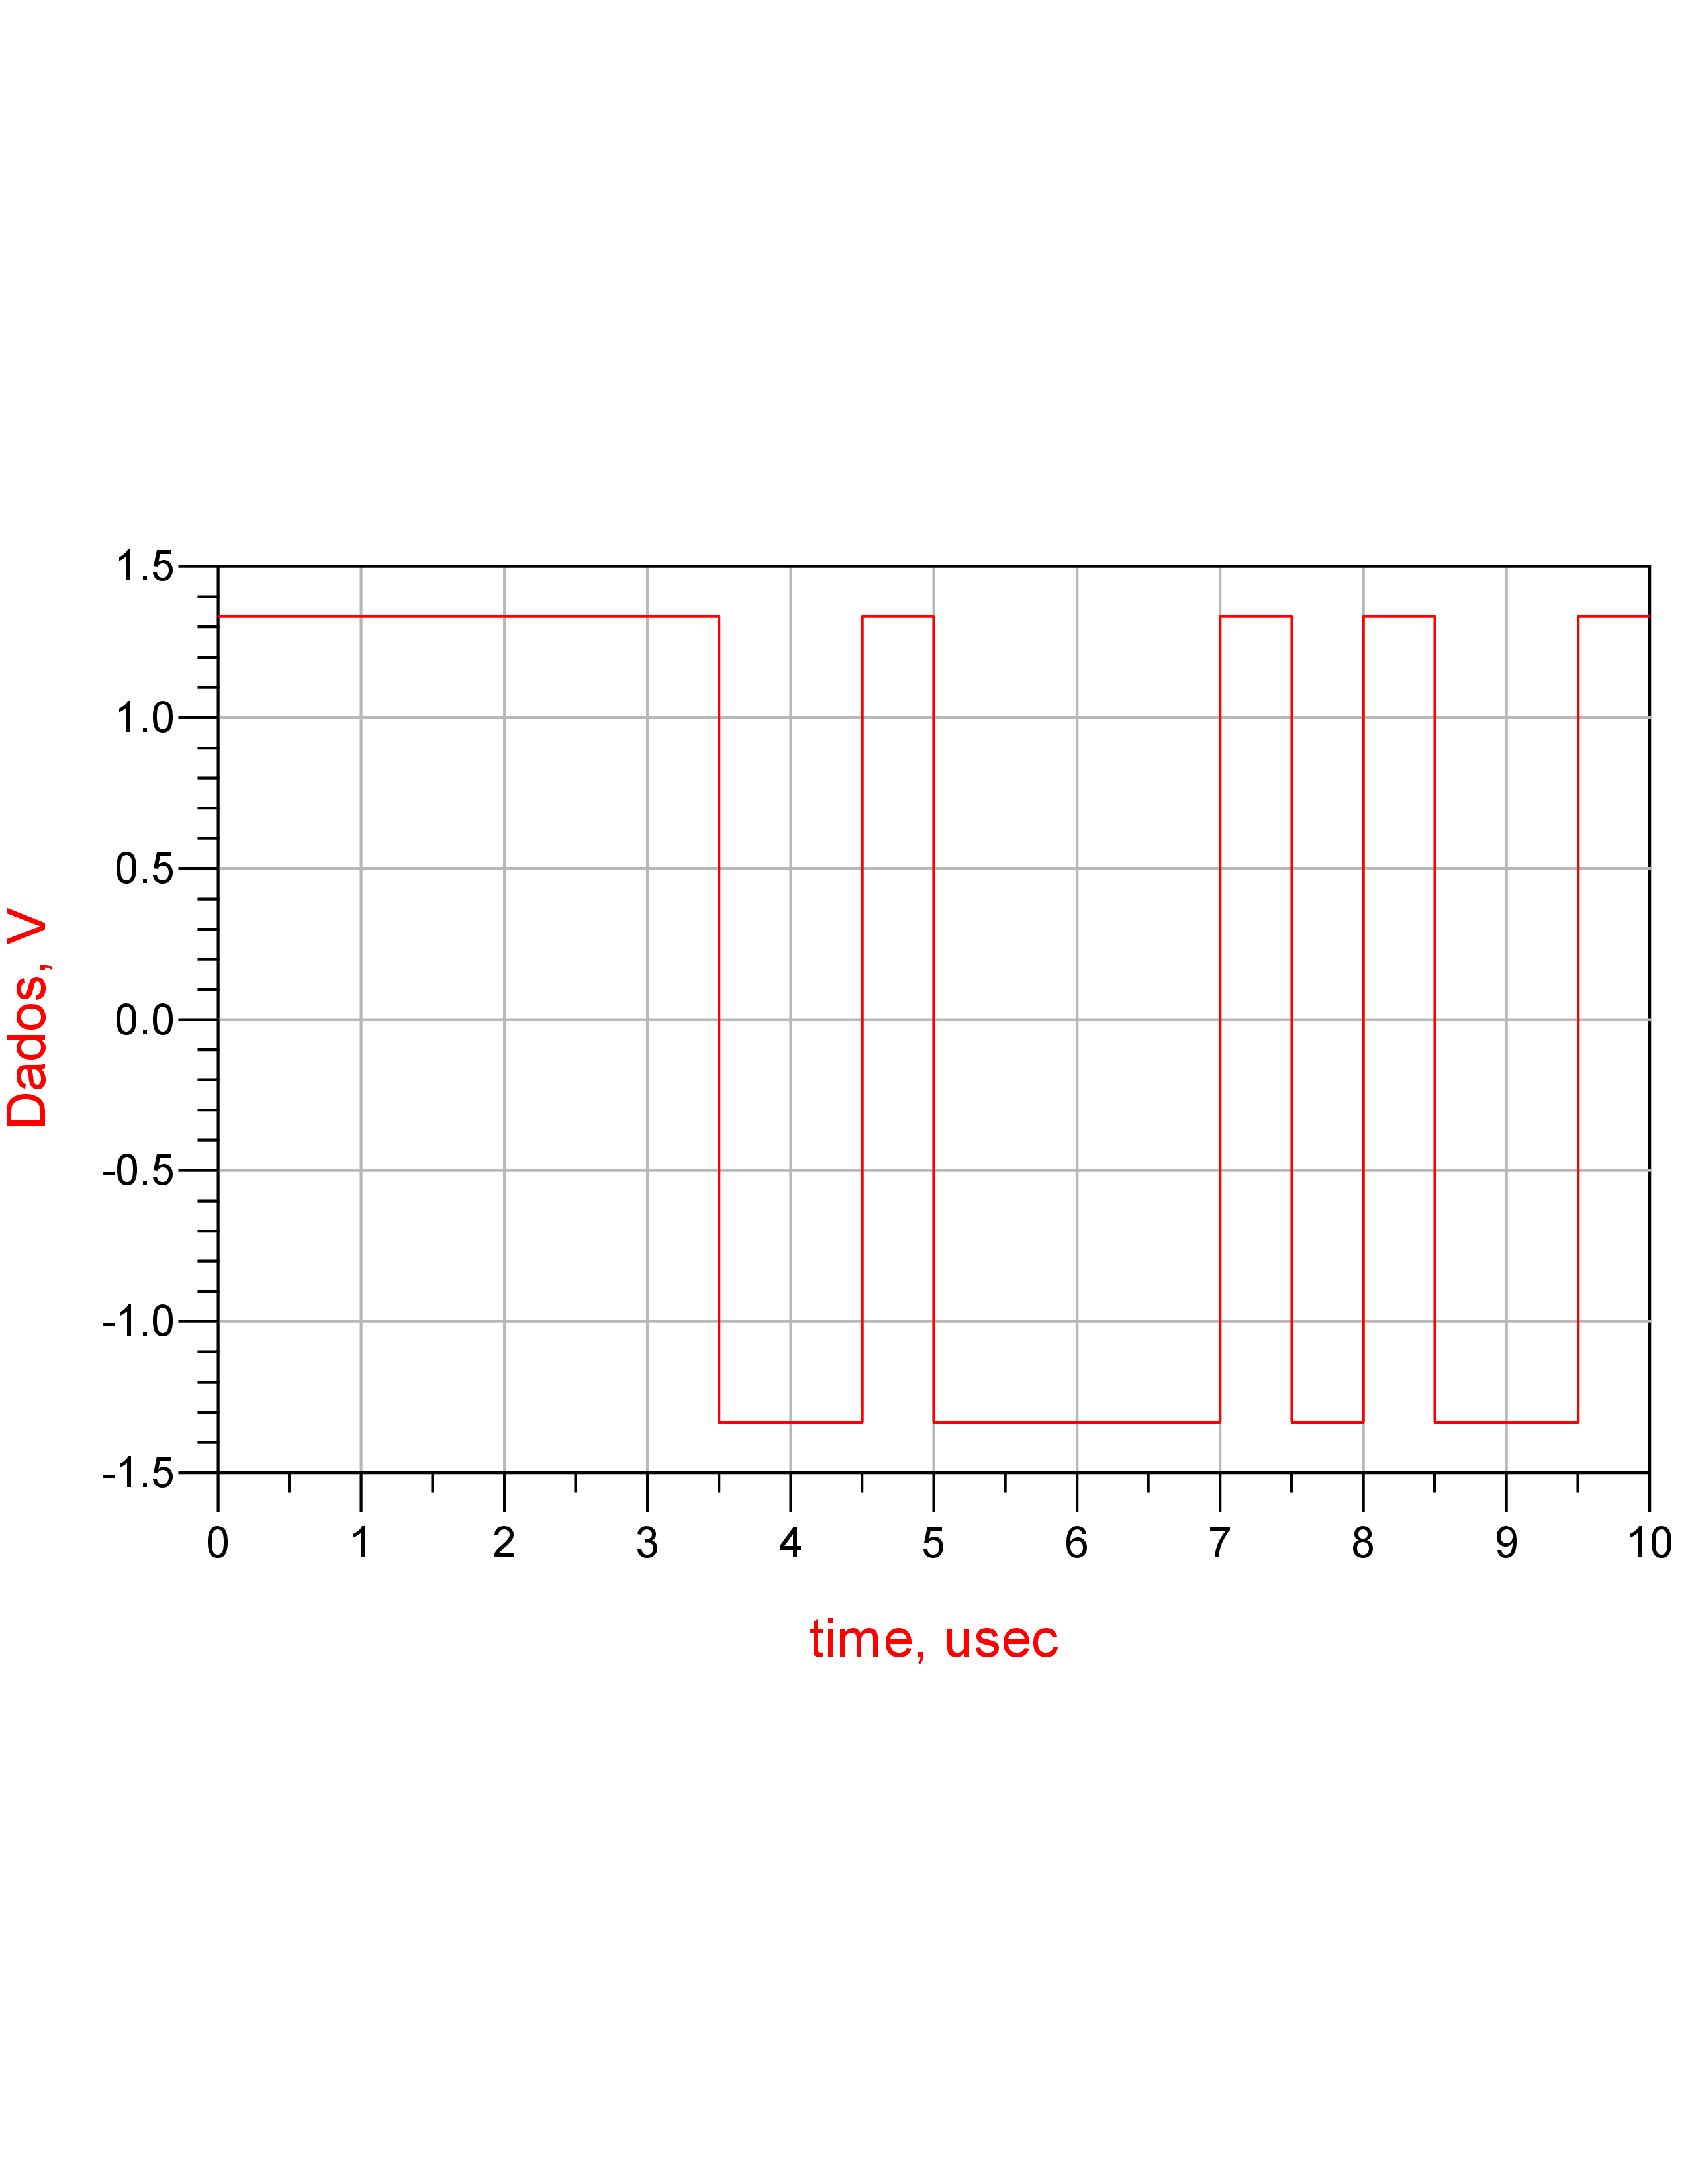
\includegraphics[width=\linewidth]{./segundo_exp/img1.png}
  \captionof{figure}{Dados gerados}
  \label{fig:test48}
\end{minipage}
\end{figure}
\begin{figure}
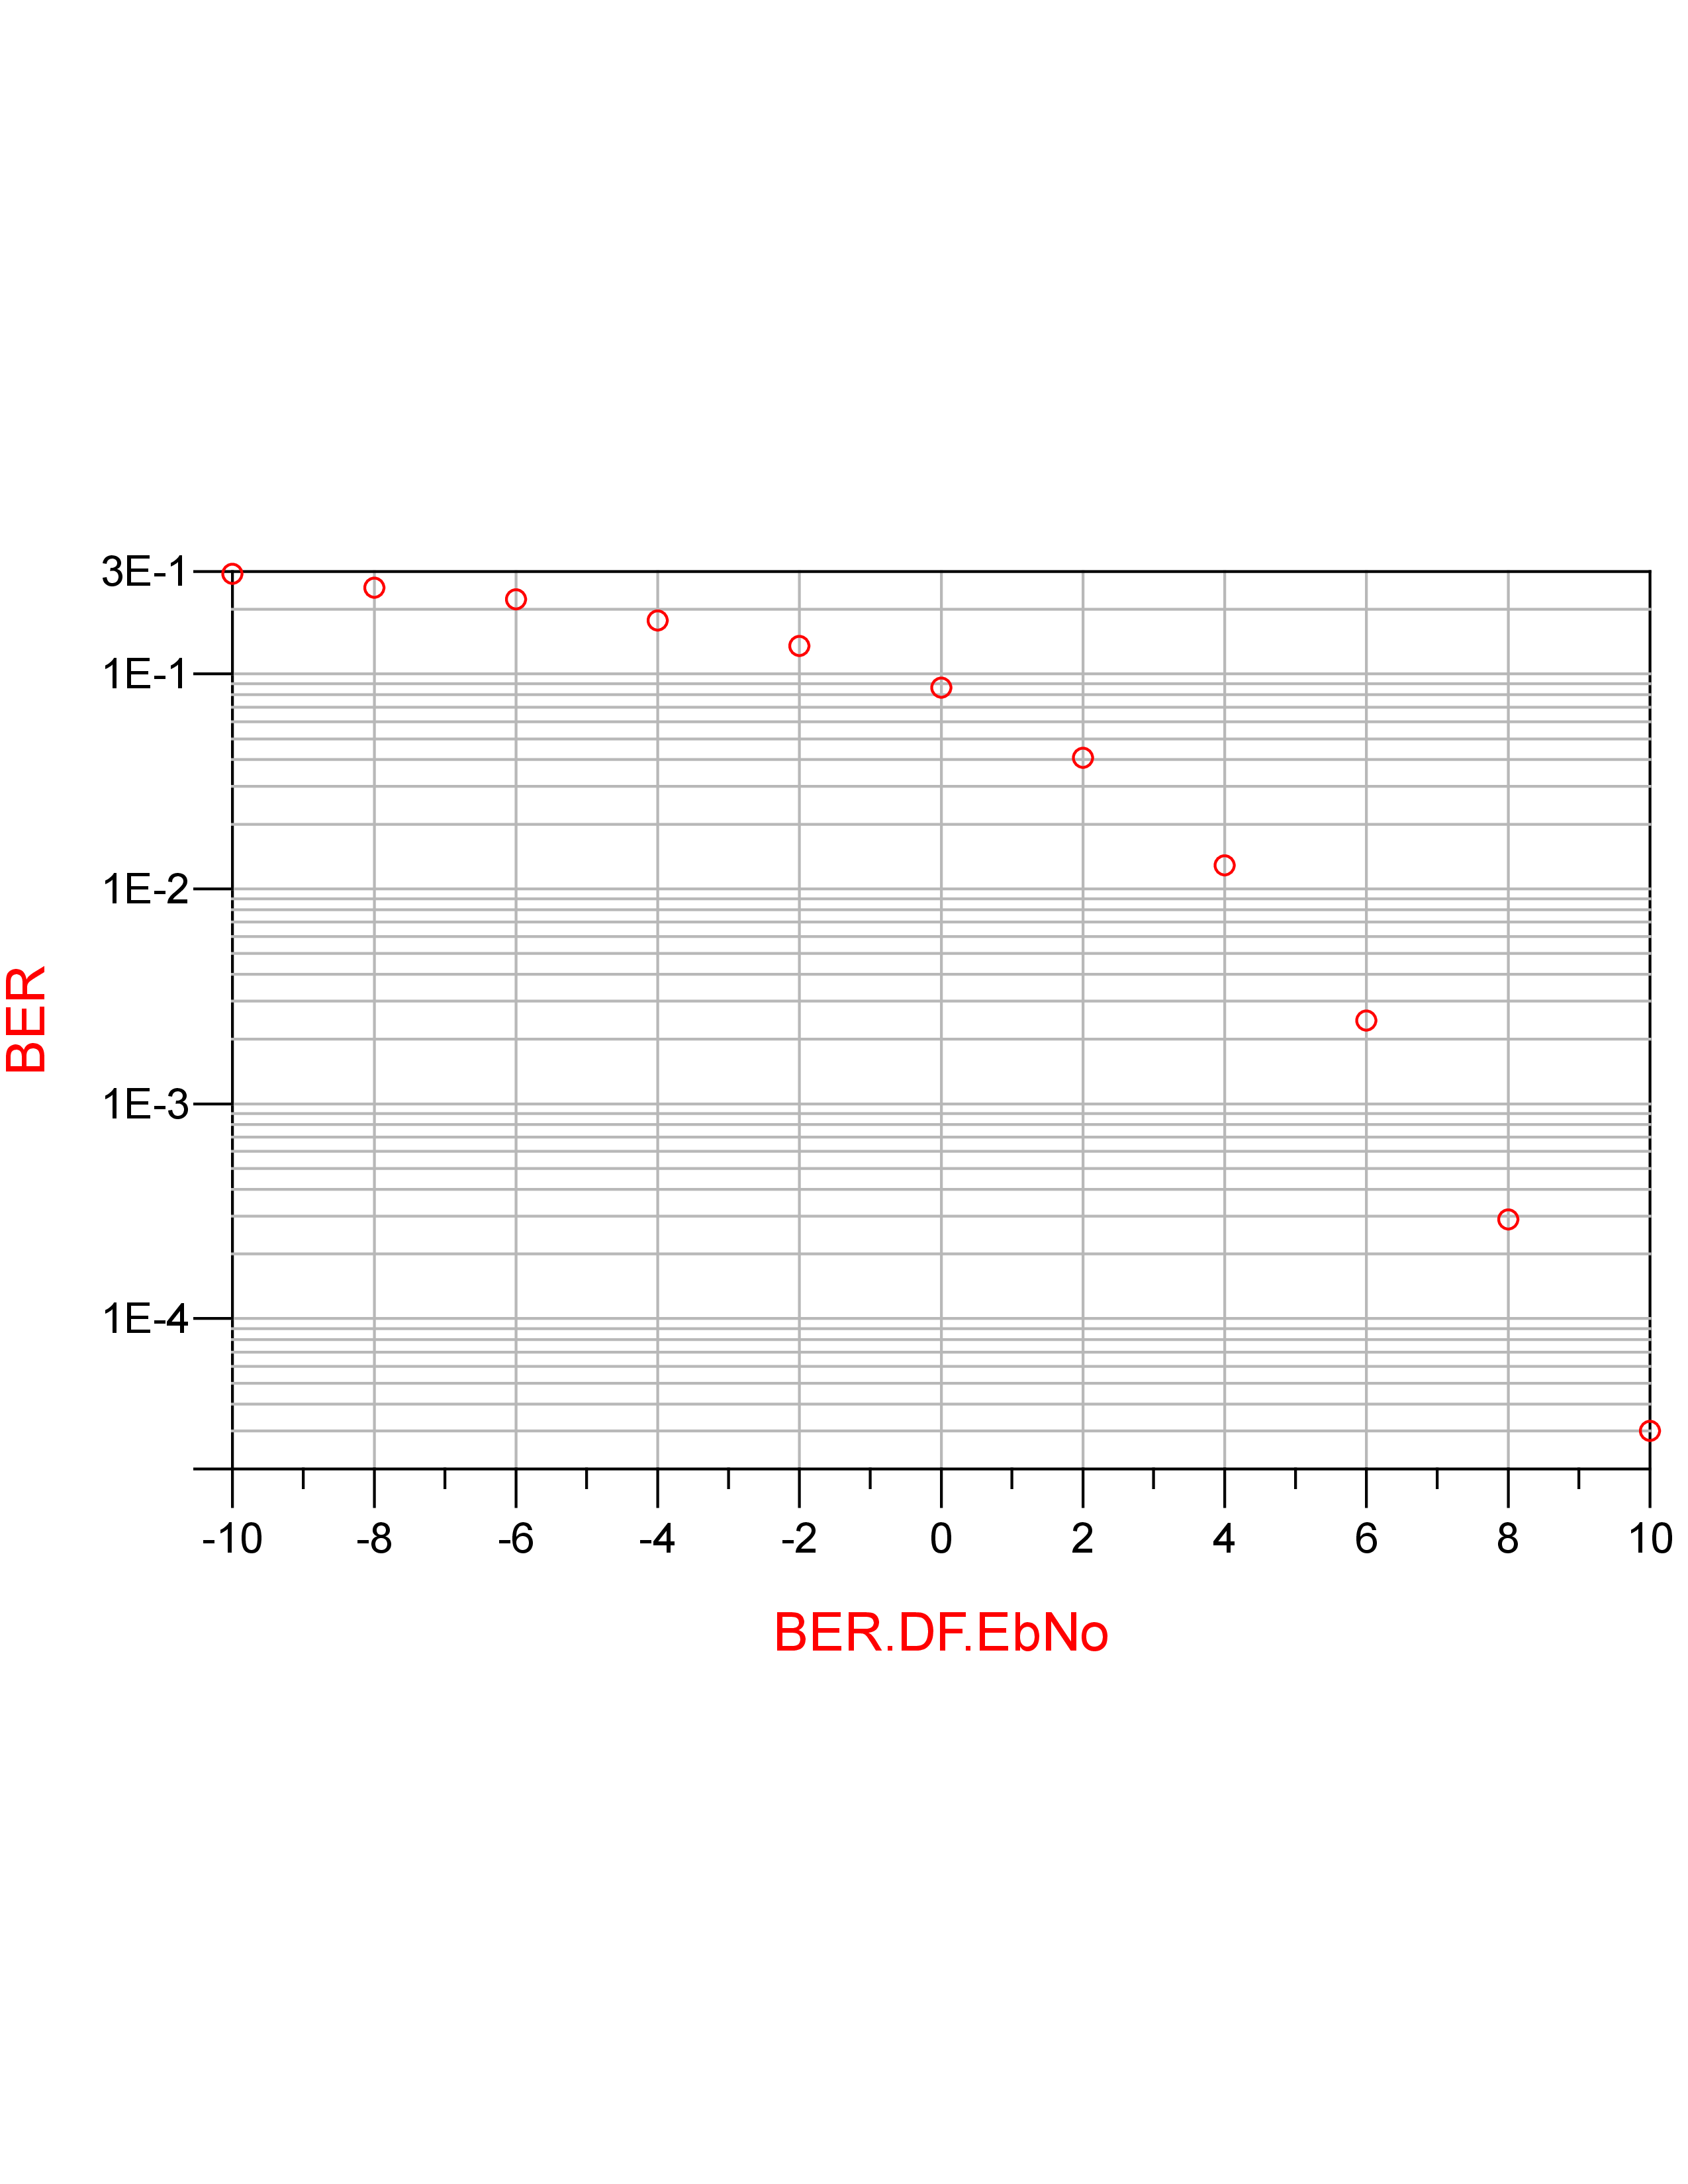
\includegraphics[width=.8\linewidth]{./segundo_exp/img7.png}
\caption{BER obtida com 1000000 pontos de simulação para vários valores de $E_b/N_o$. O valor obtido deve diferir levemente da curva teórica pois existe uma certa variância no número de bits que serão detectados de forma errada e esta variância deve pesar no cálculo da BER. A medida que o número de bits transmitidos aumenta, mais a curva obtida se aproxima da curva teórica}
\end{figure}
\begin{figure}
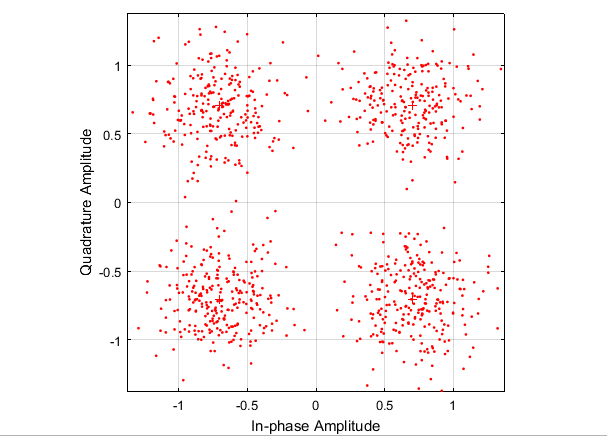
\includegraphics[width=.8\linewidth]{./segundo_exp/img8.png}
\caption{Espalhamento dos pontos da Constelação QPSK em forma de nuvem devido ao ruído AWGN. A figura utilizada foi gerada no MATLAB e é meramente ilustrativa pois nos esquecemos de retirar a figura correspondente ao ADS. Usamos 1000 pontos com uma SNR de 9dB de forma a ilustrar o conceito do surgimento de uma nuvem em torno dos pontos de referência da constelação.}
\end{figure}
